\chapter{The \thinkhomeweather ontology}
\label{ch:thinkhomeweather_ontology}

% TODO put all names of steps according to \methontology into \emph
% TODO mention - this chapter does not cover the ontology development process as it was done; instead, it presents the completed documents that were created in that processs.
% TODO mention second paper about methontology (the one that describes all artefacts created when building the chemical ontology)

% TODO check if the things mentioned here are properly covered in the chapters referred

% TODO rename: belongsToWeatherReport -> belongsToReport

% TODO elaborate steps more?

% TODO reference paper: Building legal ontologies with METHONTOLOGY and WebODE

The previous chapters cover all topics that require discussion before being able to build a new ontology from scratch: Chapter \ref{ch:weather_data} discusses all details about weather data that is necessary and reasonable for the \thinkhomeweather ontology, what data will be used and where to obtain it. Chapter \ref{ch:existing_work} gives an overview about existing ontologies in the domain of weather data. As none of the existing ontologies being discussed fits the needs of an ontology for \thinkhome, a new ontology is to be designed. Chapter \ref{ch:development_approaches} analyzes some of the most popular approaches for building ontologies from scratch. Among those, \methontology \cite{Methontology} is identified to be the best suitable approach.

Based on these insights, this chapter describes the process of designing the \thinkhomeweather ontology in detail. The development process follows the steps proposed by \methontology as described in chapter \ref{sec:methontology}.

\section{Conventions}
\label{sec:ontology_conventions}

\begin{figure}
  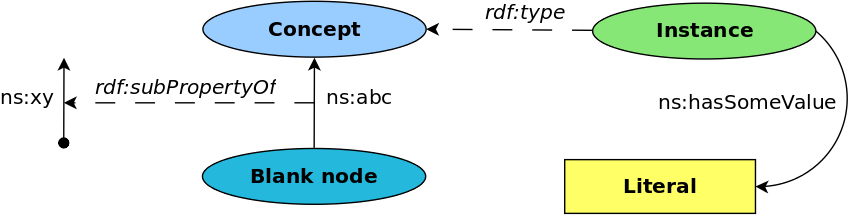
\includegraphics[width=\textwidth]{figures/diagrams/template.png}
  \caption{Example diagram}
  \label{fig:diagram_example}
\end{figure}

\definecolor{convention_color1}{HTML}{99CCFF}
\definecolor{convention_color2}{HTML}{87E776}
\definecolor{convention_color3}{HTML}{23B8DC}
\definecolor{convention_color4}{HTML}{FFFF66}
\definecolor{convention_color_bg4}{HTML}{AAAAAA}

All diagrams in this chapter showing parts of an ontology adhere to the following conventions, as seen in the example diagram shown in figure \ref{fig:diagram_example}:
\begin{itemize}
  \item \emph{Concepts} are drawn as ellipses filled with the color \texttt{\textcolor{convention_color1}{\#99CCFF}}.
  \item \emph{Instances} are drawn as ellipses filled with the color \texttt{\textcolor{convention_color2}{\#87E776}}.
  \item \emph{Blank nodes} are drawn as ellipses filled with the color \texttt{\textcolor{convention_color3}{\#23B8DC}}.
  \item \emph{Literals} are drawn as rectangles filled with the color \texttt{\colorbox{convention_color_bg4}{\textcolor{convention_color4}{\#FFFF66}}}.
  \item \emph{Properties in the RDF\cite{RDF} and RDFS\cite{RDFS} namespace} are drawn as dashed lines. Their caption is written in \emph{italics}.
  \item \emph{Properties in other namespaces} are drawn as solid lines. Their caption is \emph{not} written in \emph{italics}.
\end{itemize}

% TODO cite chapter 6 of OWL 101?
The naming conventions for identifiers within the ontology are as follows:
\begin{itemize}
  \item Two concepts, instances and/or properties may not have the same identifier as this is required by \emph{OWL}\cite{OWL}\footnote{Using one identifier for more than one concept, instance and properties is possible in \emph{OWL} if an adequate number of namespaces is used. However, \thinkhomeweather uses a single namespace.} and avoids confusion.
  \item Two identifiers may not use names that only differ in their capitalization. Using both \emph{Weather State} and \emph{weather state} in the name namespace is possible in \emph{OWL}, but leads to confusion.
  \item Identifiers may only consist of upper and lower case ASCII letters (\emph{A} to \emph{Z} and \emph{a} to \emph{z}), numerical digits from \emph{0} to \emph{9} and spaces, i.e. all identifiers must match the regular expression \texttt{\textasciicircum[A-za-z0-9~]+\$}.
  \item \emph{Concepts} have an identifier that is in singular case and starts with an upper case letter. Typically a concept's identifier is a noun, e.g. \emph{Weather state} or \emph{Weather report}.
  \item \emph{Properties} have an identifier that starts with a lower case letter and starts with the prefix \emph{has} or \emph{belongs to}, followed by the name of the name of the concept which is the property's \emph{range}. The inverse property of a property having an identifier starting with \emph{has} has an identifier starting with \emph{belongs to}, followed by the inverse property's \emph{range}, and vice versa. As an alternative to the prefix \emph{belongs to}, the prefix \emph{is} in conjunction with the suffix \emph{of} and the inverse property's \emph{domain} may be used.
  
  E.g. the name of a property with the domain \emph{Weather report} and the range \emph{Weather state} has the name \emph{has weather state}. If \emph{has weather state} has an inverse property, it will have the name \emph{belongs to weather report} or \emph{is weather state of}.
\end{itemize}


\section{Specification}
\label{sec:ontology_specification}

% TODO put document template in other chapter
\emph{Specification}, the first step proposed by \methontology, aims at creating an \emph{Ontology Requirements Specification Document} using natural language. It adheres to the approach discussed in chapter \ref{sec:methontology} and uses the document template taken from \cite{ORSD}.

\vspace{1em}

% TODO ensure there are no problematic page breaks inside this box (e.g. between the headline 'Scope:' and the first bullet point)
\begin{mdframed}[linewidth=.6pt]
\setlength{\parindent}{0pt}
\vspace{.3cm}

\MakeUppercase{\textbf{Ontology Requirements Specification Document}}

\vspace{.5cm}

\textbf{Name}: \thinkhomeweather

\vspace{.2cm}

\textbf{Purpose}: The ontology covers data about weather phenomena occurring at a certain location somewhere on Earth between the present and 24 hours in the future. Weather data will be acquired from both Internet services as well as from weather sensors mounted at the desired location. This weather data will enable the \thinkhome system to make decisions based on current and future weather conditions.

\vspace{.2cm}

\textbf{Scope}: The ontology has to cover a set of six core concepts from the domain of weather data:

\begin{itemize}
  \item \emph{weather phenomenon}: Represents a certain weather element. Relevant weather elements are \emph{temperature}, \emph{humidity}, \emph{dew point}, \emph{wind speed} and \emph{direction}, \emph{precipitation intensity} and \emph{probability}, \emph{atmospheric pressure}, \emph{cloud cover}, \emph{solar radiation}, and the \emph{sun's position}.
  \item \emph{Weather condition}: Overall state of the weather given by a simple verbal description: \emph{sun}, \emph{light clouds}, \emph{partly cloudy}, \emph{cloudy}, \emph{fog}, \emph{rain}, \emph{snow}, \emph{sleet}, \emph{thunder}.
  \item \emph{Weather state}: Summarizes all weather phenomena for a certain time. 
  \item \emph{Weather report}: Summarizes all data acquired at a certain time about the current weather or the weather some time in the future. Exactly one \emph{weather state} is linked to each \emph{weather report}.
  \item \emph{Weather report source}: Source where the data belonging to a \emph{weather report} has been obtained from (either an Internet weather service or a local weather sensor).
\end{itemize}

\vspace{.2cm}

\textbf{Implementation language}: The ontology is implemented in \emph{OWL 2.0}\cite{OWL} using \protege\footnote{\href{http://protege.stanford.edu/}{http://protege.stanford.edu/}} and the \emph{Pellet reasoner}\footnote{\href{http://clarkparsia.com/pellet/}{http://clarkparsia.com/pellet/}}.

\vspace{.2cm}

% TODO reformulate
\textbf{Intended end-users}: The ontology is part of the \thinkhome project. Hence, any user of the \thinkhome project is a user of the \thinkhomeweather ontology. \thinkhome aims at providing home automation to \emph{house occupants}; therefore, every occupant of a house is a possible end user for \thinkhomeweather. However, he/she will never have to deal with any ontology. \thinkhome is ought to make decisions on itself based on the knowledge acquired from the \thinkhomeweather ontology. Only the \emph{developers of \thinkhome} have to deal with the ontology itself.

\vspace{.2cm}

\textbf{Intended uses}: The ontology shall provide knowledge to \thinkhome about the current and future state of the weather in order to enable \thinkhome to make decisions based on that knowledge.

\vspace{.2cm}

\textbf{Ontology requirements}:

\vspace{.2cm}

\setlength{\leftskip}{.5cm}

\textbf{Non-functional requirements}:

\begin{itemize}
  \item The ontology must adhere to the naming conventions presented in section \ref{sec:ontology_conventions} regarding the identifiers that may be used for classes, properties and individuals.
  \item The ontology must be documented thoroughly in order to make it easily reusable.
  \item The ontology must re-use existing ontologies wherever possible.
\end{itemize}

\textbf{Functional requirements}: The functional requirements are covered by the competency questions that the ontology shall be able to answer (see section \ref{sec:weather_information}):

\begin{itemize}
  \item What is the current weather situation?
  \item What will the weather situation be in one hour, in two hours, …, in 24 hours?
  \item What is the current temperature, humidity, wind speed, …?
  \item What will be the temperature, humidity, wind speed, … in one hour, in two hours, …, in 24 hours?
  \item What will be the minimum temperature, humidity, … over the next 24 hours? What about maximum values?
  \item Will the weather change? Will the temperature, humidity, … rise or fall?
  \item Does it rain? Will it rain in the next hours? Will it rain today?
  \item Will there be sunshine today? 
  \item Do we need to irrigate the garden?
  \item Will there be severe weather?
  \item Will temperature drop/stay below $0^\circ C$?
  \item When can we open windows and when do we have to keep them shut?
  \item When do we need sun protection?
  \item When will it outside be colder than inside the house? When will it be warmer?
\end{itemize}

\setlength{\leftskip}{0cm}

\vspace{.2cm}

\textbf{Pre-glossary of terms}: These are all terms that can be extracted from the competency questions, in alphabetical order:

24 hours, airing, current weather, frost, future weather, humidity, humidity rise, humidity fall, irrigation, minimum, maximum, rain, room temperature, severe weather, sunshine, sun protection, temperature, temperature rise, temperature fall, weather change, wind speed.

\setlength{\leftskip}{0cm}

\end{mdframed}

\vspace{.5cm}

In the following sections, the \thinkhomeweather ontology is built in a way to meet all above requirements, if possible. Section \ref{sec:ontology_evaluation} evaluates if the resulting ontology fits the specification and which shortcomings the ontology comes with.

\section{Knowledge Acquisition}

The second step proposed by \methontology is \emph{Knowledge Acquisition}. All knowledge required to build the \thinkhomeweather ontology is presented in the chapters~\ref{ch:existing_work} and~\ref{ch:weather_data}. These chapters discuss in detail:

\begin{itemize}
  \item Which weather data are relevant for \thinkhome?
  \item Which weather data are available from sensors (section~\ref{sec:weather_sensors}) and Internet services (section~\ref{sec:internet_services})? How can this data be acquired?
  \item Which data do not have any use for \thinkhomeweather due to being too complicated or because they cannot be processed in an ontology in a useful way?
  \item What knowledge about weather in general is required to build an appropriate ontology? % TODO check if this is available in the previous chapters
\end{itemize}

Furthermore, chapter~\ref{ch:existing_work} covers existing ontologies that cover the domain of weather data. An additional source of knowledge is available through works about weather in general, e.g. the \emph{Glossary of Meteorology}\footnote{\href{http://glossary.ametsoc.org/wiki/Main\_Page}{http://glossary.ametsoc.org/wiki/Main\_Page}} by the \emph{American Meteorological Society}\footnote{\href{http://www.ametsoc.org/}{http://www.ametsoc.org/}}\cite{GlossaryOfMeteorology}.

\section{Conceptualisation}

In the third step of \methontology, the \emph{Conceptualisation} step, the domain knowledge is structured into a conceptional model that describes the problem and its solution in terms of the domain vocabulary that has been identified in the \emph{Specification} process.

The starting point of \emph{Conceptualisation} is a complete \emph{Glossary of Terms} that covers all concepts, instances, attributes and binary relations that will form the ontology. Besides the glossary, this section covers \emph{Concept-classification trees} (section~\ref{sec:concept_classification_trees}), \emph{Binary relationship diagrams} (section~\ref{subsec:binary_relations_diagram}), \emph{Concept dictionaries} (section~\ref{subsec:binary_relations_diagram}), \emph{Binary relations tables} (section~\ref{subsec:binary_relations_table}), \emph{Instance attribute tables} (section~\ref{subsec:binary_relations_table}) and \emph{Class attribute tables} (section~\ref{subsec:class_attribute_tables}). \emph{Constant tables}, \emph{Formal axiom tables} and \emph{Rules tables} have been omitted as the components described by these tables do not appear in \thinkhomeweather.

In this section, only those deliverables are presented that are necessary to fully understand the structure of \thinkhomeweather. All tables that have only been created for the sake of completeness can be found in appendix~\ref{sec:appendix_conceptualisation}.

\subsection{Glossary of Terms}
\label{sec:ontology_glossary}

When describing the scope of \thinkhomeweather, the \emph{Ontology Requirements Specification Document} in section~\ref{sec:ontology_specification} mentions five top-level concepts (i.e. concepts that do not have a superclass except \emph{Thing} in \emph{OWL}) of the ontology: \Egls{weather report}, \Egls{weather state}, \Egls{weather phenomenon}, and \Egls{weather condition}. All other concepts are sub-concepts of these five concepts.

In this section, only a list of terms is given; the complete \emph{Glossary of Terms} with short descriptions of each term can be found in the appendix~\ref{main} which starts on page~\pageref{main}.

\paragraph{Concepts:}

% TODO link to section/subsection?
Section~\ref{ch:weather_data} discusses each weather element that is used in \thinkhomeweather and categories in which its instances can be grouped into. In the ontology, all weather elements are represented by concepts that sub-concepts of \Egls{weather phenomenon}. All categories of weather elements are in turn sub-concepts of the weather elements' concepts.

A \egls{weather report} can encapsulate data either about the current weather or about the weather some time in the future which is specified by its \egls{start time}. Additionally, weather data can origin at a set of weather sensors or at an Internet weather service. To take this into account, a few sub-concepts of \egls{weather report} are introduced:

If the \egls{weather report} describes the current weather, it is a \Egls{current weather report}; if it describes the future weather, it is a \Egls{forecast weather report}. Depending on how far the \Egls{weather report}'s \egls{start time} lies into the future, it is a \Egls{short range weather report} (at most 3 hours in the future), a \Egls{medium range weather report} (more than 3 hours and less than 12 hours in the future) or a \Egls{long range weather report} (at least 12 hours in the future). % TODO additional concepts

If the source of weather data is a \Egls{sensor source}, the corresponding \Egls{weather report} is a \Egls{weather report from sensor}; otherwise (if the source of weather data is a \Egls{service source}), it is a \Egls{weather report from service}.

A \Egls{weather report} that is both a \Egls{current weather report} and a \Egls{weather report from sensor} is a \Egls{current weather report from sensor}. A \Egls{weather report} that is both a \Egls{current weather report} and a \Egls{weather report from service} is a \Egls{current weather report from service}.

% TODO additional sub-concepts of Weather states

Hence, these are the concepts that can be found in \thinkhomeweather are:
\begin{itemize}
  \item \Egls{weather condition}
  \item \Egls{weather phenomenon}:
    \begin{itemize}
      \item \Egls{atmospheric pressure}: \Egls{very low pressure}, \Egls{low pressure}, \Egls{average pressure}, \Egls{high pressure}, \Egls{very high pressure}
      \item \Egls{cloud cover}: \Egls{clear sky}, \Egls{partly cloudy}, \Egls{mostly cloudy}, \Egls{overcast}, \Egls{unknown cloud cover}.
      \item \Egls{dew point}.
      \item \Egls{humidity}: \Egls{very dry}, \Egls{dry}, \Egls{normal humidity}, \Egls{moist}, \Egls{very moist}.
      \item \Egls{precipitation}: \Egls{no rain}, \Egls{light rain}, \Egls{medium rain}, \Egls{heavy rain}, \Egls{extremely heavy rain}, \Egls{tropical storm rain}.
      \item \Egls{solar radiation}: \Egls{no radiation}, \Egls{low radiation}, \Egls{medium radiation}, \Egls{high radiation}, \Egls{very high radiation}.
      \item \Egls{sun position}: \Egls{day}, \Egls{solar twilight}, \Egls{sun below horizon}, \Egls{twilight}, \Egls{civil twilight}, \Egls{nautical twilight}, \Egls{astronomical twilight}, \Egls{night}, \Egls{sun from north}, \Egls{sun from east}, \Egls{sun from south}, \Egls{sun from west}.
      \item \Egls{temperature}: \Egls{frost}, \Egls{cold}, \Egls{below room temperature}, \Egls{room temperature}, \Egls{above room temperature}, \Egls{heat}.
      \item \Egls{wind}: \Egls{directional wind}, \Egls{north wind}, \Egls{east wind}, \Egls{south wind}, \Egls{west wind}, \Egls{calm}, \Egls{light wind}, \Egls{strong wind}, \Egls{storm}, \Egls{hurricane}.
    \end{itemize}
  \item \Egls{weather report}: \Egls{weather report from sensor}, \Egls{weather report from service}, \Egls{current weather report}, \Egls{current weather report from sensor}, \Egls{current weather report from service}, \Egls{forecast weather report}, \Egls{short range weather report}, \Egls{medium range weather report}, \Egls{long range weather report} % TODO additional concepts
  \item \Egls{weather source}: \Egls{sensor source}, \Egls{service source}.
  \item \Egls{weather state} % TODO additional concepts
\end{itemize}

\paragraph{Relations:}

Instances of the concepts are associated to each other with binary relations, which are:

\begin{itemize}
  \item \egls{has source} and \egls{is source of} which connect instances of \Egls{weather report} and \Egls{weather source}.
  \item \egls{has weather state} and \egls{belongs to weather report} which connect instances of \Egls{weather report} and \Egls{weather state}.
  \item \egls{has condition} which connects instances of \Egls{weather state} and \Egls{weather condition}.
  \item \egls{has weather phenomenon} and \egls{belongs to state} which connect instances of \Egls{weather state} and \Egls{weather phenomenon}.
  \item \egls{has previous weather state} and \egls{has next weather state} which connect two instances of \Egls{weather state}.
\end{itemize}

The following relations link instances of concepts from other ontologies than \thinkhomeweather to instances of concepts inside the ontology: \egls{has start time}, \egls{has end time}, \egls{has observation time}, and \egls{location}.

The only data property in \thinkhomeweather is \egls{has priority} which specifies an integer value indicating which \Egls{weather report} for a certain period of time is to be preferred over another \Egls{weather report} for the same period of time.

\paragraph{Individuals:}

The only predefined individuals are instances of the concept \Egls{weather condition}; they represent the overall state of the weather for a certain \Egls{weather state}. These individuals are: \emph{cloud}, \emph{fog}, \emph{light clouds}, \emph{partly cloudy}, \emph{rain}, \emph{sleet}, \emph{snow}, \emph{sun}, and \emph{thunder}.

\subsection{Concept-classification trees}
\label{sec:concept_classification_trees}

As stated in section~\ref{sec:ontology_glossary}, there are fix top-level concepts; all other concepts are sub-concepts to these top-level concepts. As a consequence, each of these concepts becomes root of a tree of concepts. These \emph{Concept-classification trees} are presented in this section.

A \Egls{weather condition} does not have any sub-concepts. Hence, its classification tree which is shown in figure~\ref{fig:tree_weather_condition} looks rather simple.

\begin{figure}
  \centering
  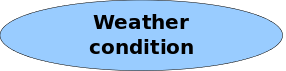
\includegraphics[width=.3\textwidth]{figures/diagrams/weather-condition.png}
  \caption{Concept-classification tree for \Egls{weather condition}}
  \label{fig:tree_weather_condition}
\end{figure}

A \Egls{weather phenomenon} represents a certain weather element. Every specific weather element is a sub-concept of \Egls{weather phenomenon}; the evolving tree is shown in~\ref{fig:tree_weather_phenomenon}. For sake of clarity, this tree is broken up to several diagrams; all sub-concepts of sub-concepts of \Egls{weather phenomenon} are not shown in~\ref{fig:tree_weather_phenomenon}. There is a separate diagram for each sub-concept of \Egls{weather phenomenon}: \Egls{atmospheric pressure} (figure~\ref{fig:tree_atmospheric_pressure}), \Egls{cloud cover} (figure~\ref{fig:tree_cloud_cover}), \Egls{humidity} (figure~\ref{fig:tree_humidity}), \Egls{precipitation} (figure~\ref{fig:tree_precipitation}), \Egls{solar radiation} (figure~\ref{fig:tree_solar_radiation}), \Egls{sun position} (figure~\ref{fig:tree_sun_position}), \Egls{temperature} (figure~\ref{fig:tree_temperature}), and \Egls{wind} (figure~\ref{fig:tree_wind}). The diagram for \Egls{dew point} is not shown as that concept does not have any sub-concepts; hence its concept-classification tree consists of a single node.

\begin{figure}
  \centering
  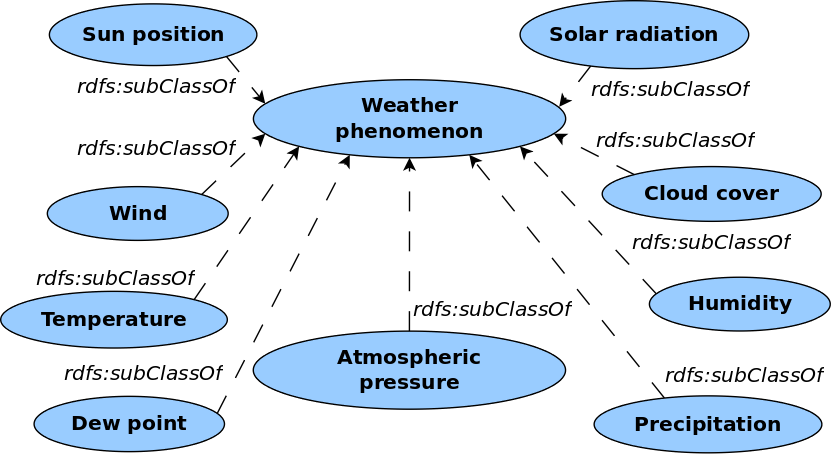
\includegraphics[width=.8\textwidth]{figures/diagrams/weather-phenomenon.png}
  \caption{Concept-classification tree for \Egls{weather phenomenon}}
  \label{fig:tree_weather_phenomenon}
\end{figure}

\begin{figure}
  \centering
  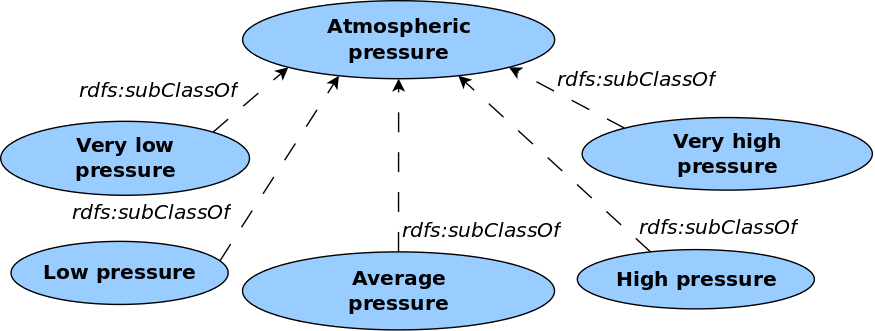
\includegraphics[width=.8\textwidth]{figures/diagrams/atmospheric-pressure.png}
  \caption{Concept-classification tree for \Egls{atmospheric pressure}}
  \label{fig:tree_atmospheric_pressure}
\end{figure}

\begin{figure}
  \centering
  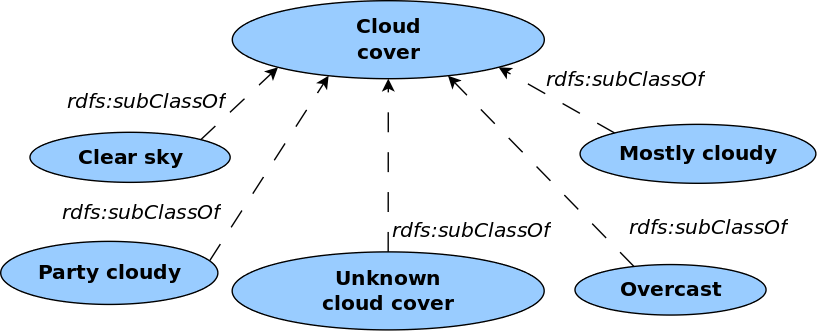
\includegraphics[width=.8\textwidth]{figures/diagrams/cloud-cover.png}
  \caption{Concept-classification tree for \Egls{cloud cover}}
  \label{fig:tree_cloud_cover}
\end{figure}

\begin{figure}
  \centering
  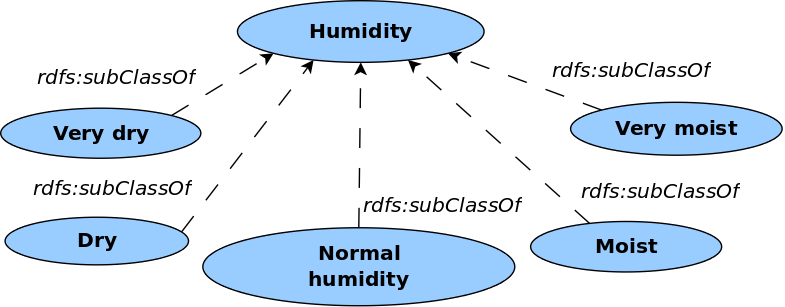
\includegraphics[width=.8\textwidth]{figures/diagrams/humidity.png}
  \caption{Concept-classification tree for \Egls{humidity}}
  \label{fig:tree_humidity}
\end{figure}

\begin{figure}
  \centering
  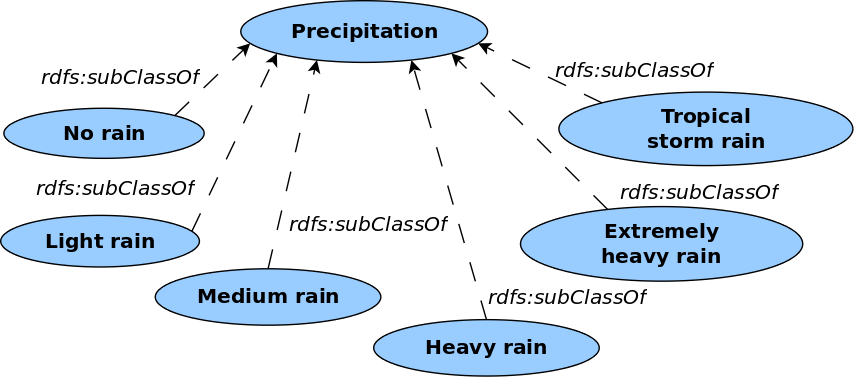
\includegraphics[width=.8\textwidth]{figures/diagrams/precipitation.png}
  \caption{Concept-classification tree for \Egls{precipitation}}
  \label{fig:tree_precipitation}
\end{figure}

\begin{figure}
  \centering
  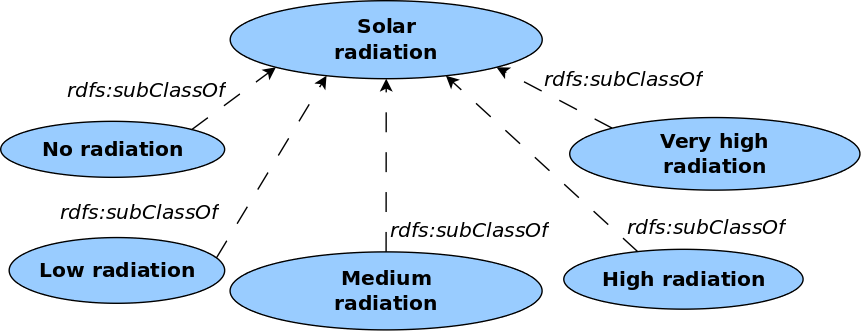
\includegraphics[width=.8\textwidth]{figures/diagrams/solar-radiation.png}
  \caption{Concept-classification tree for \Egls{solar radiation}}
  \label{fig:tree_solar_radiation}
\end{figure}

\begin{figure}
  \centering
  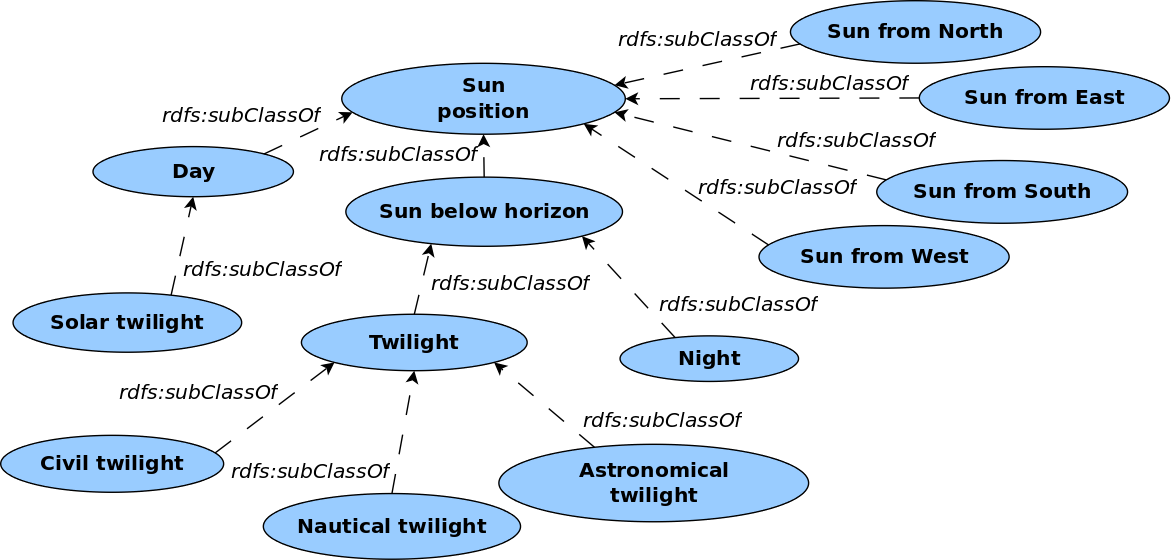
\includegraphics[width=.8\textwidth]{figures/diagrams/sun-position.png}
  \caption{Concept-classification tree for \Egls{sun position}}
  \label{fig:tree_sun_position}
\end{figure}

\begin{figure}
  \centering
  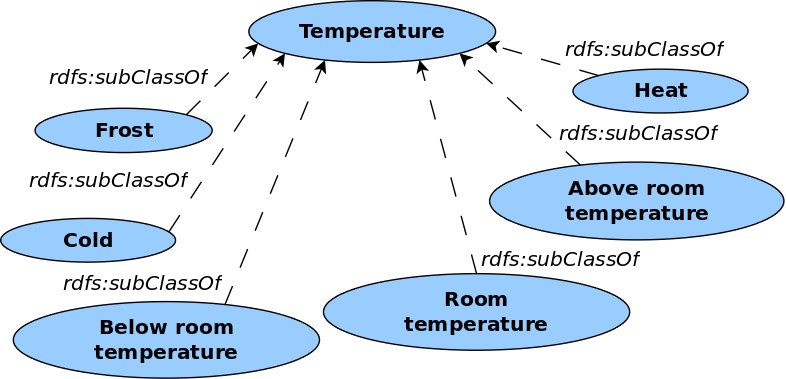
\includegraphics[width=.8\textwidth]{figures/diagrams/temperature.png}
  \caption{Concept-classification tree for \Egls{temperature}}
  \label{fig:tree_temperature}
\end{figure}

\begin{figure}
  \centering
  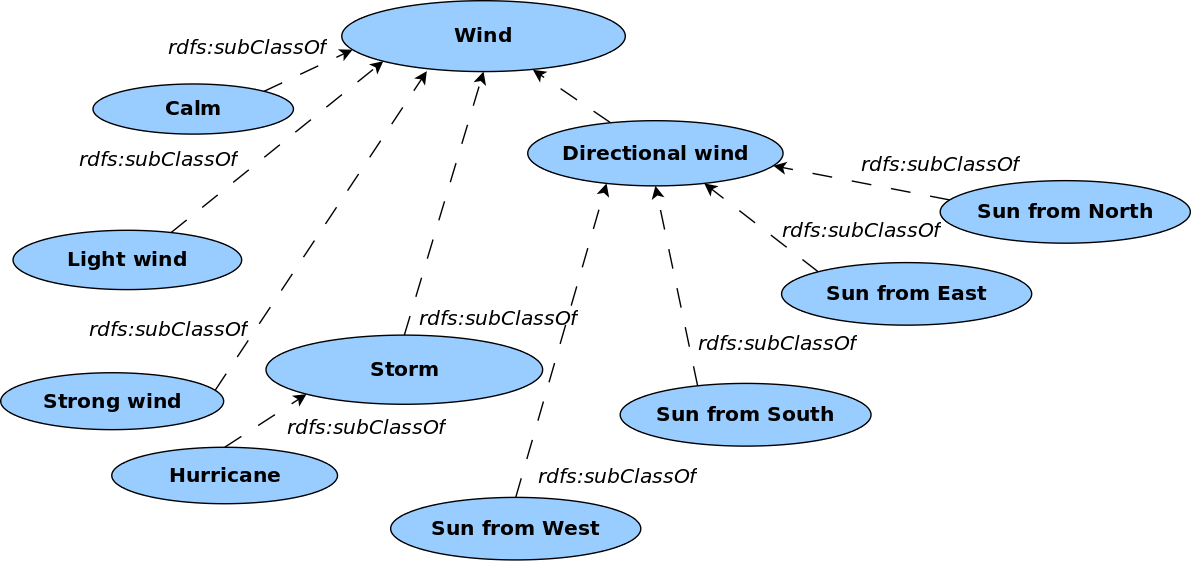
\includegraphics[width=\textwidth]{figures/diagrams/wind.png}
  \caption{Concept-classification tree for \Egls{wind}}
  \label{fig:tree_wind}
\end{figure}

A \Egls{weather report} has two attributes that define its main characteristics: \egls{has start time} and \egls{has source}. As discussed in section~\ref{sec:ontology_glossary}, a number of sub-concepts is defined in order to reflect different values of these two attributes. The resulting concept-classification tree is shown in figure~\ref{fig:tree_weather_report}.

\begin{figure}
  \centering
  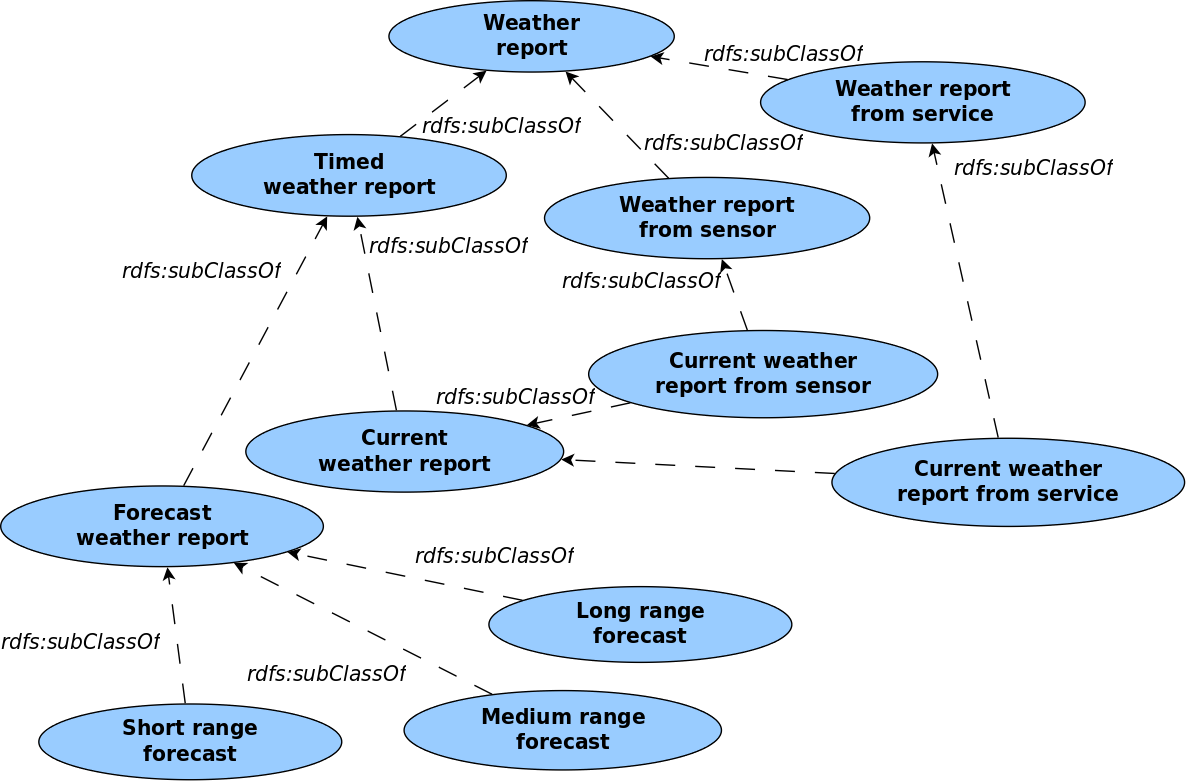
\includegraphics[width=\textwidth]{figures/diagrams/weather-report.png}
  \caption{Concept-classification tree for \Egls{weather report}}
  \label{fig:tree_weather_report}
\end{figure}

The concepts \Egls{short range weather report}, \Egls{medium range weather report} and \Egls{long range weather report} each do have sub-concepts which have been omitted from the above diagram for clarity. These sub-concepts are:
\begin{itemize}
  \item \Egls{short range weather report}: \emph{Forecast 1 hour weather report}, \emph{Forecast 2 hours weather report} and \emph{Forecast 3 hours weather report} for weather reports describing the weather in one, two and three hours, respectively.
  \item \Egls{medium range weather report}: \emph{Forecast 6 hour weather report} and \emph{Forecast 9 hours weather report} for weather reports describing the weather in 6 and 9 hours, respectively.
  \item \Egls{long range weather report}: \emph{Forecast 12 hour weather report}, \emph{Forecast 15 hours weather report}, \emph{Forecast 18 hours weather report}, \emph{Forecast 21 hours weather report} and \emph{Forecast 24 hours weather report} for weather reports describing the weather in 12, 15, 18, 21 and 24 hours, respectively.
\end{itemize}

A \Egls{weather source} can either be a \Egls{sensor source} or a \Egls{service source} (see figure~\ref{fig:tree_weather_source}).

\begin{figure}
  \centering
  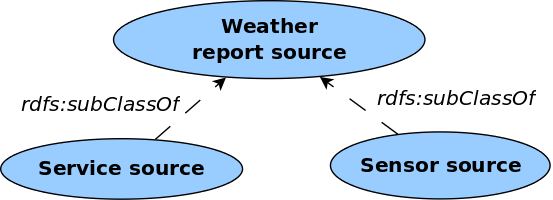
\includegraphics[width=.5\textwidth]{figures/diagrams/weather-report-source.png}
  \caption{Concept-classification tree for \Egls{weather source}}
  \label{fig:tree_weather_source}
\end{figure}

A \Egls{weather state} represents the set of weather phenomena that belong to a certain \Egls{weather report}. In order to emphasise certain combinations of instances of \Egls{weather phenomenon} being linked to the same instance of \Egls{weather state}, several sub-concepts of \Egls{weather state} are introduced (see figure~\ref{fig:tree_weather_state}): % TODO mention concepts and add them to the glossary

\begin{figure}
  \centering
  % TODO diagram is incomplete
  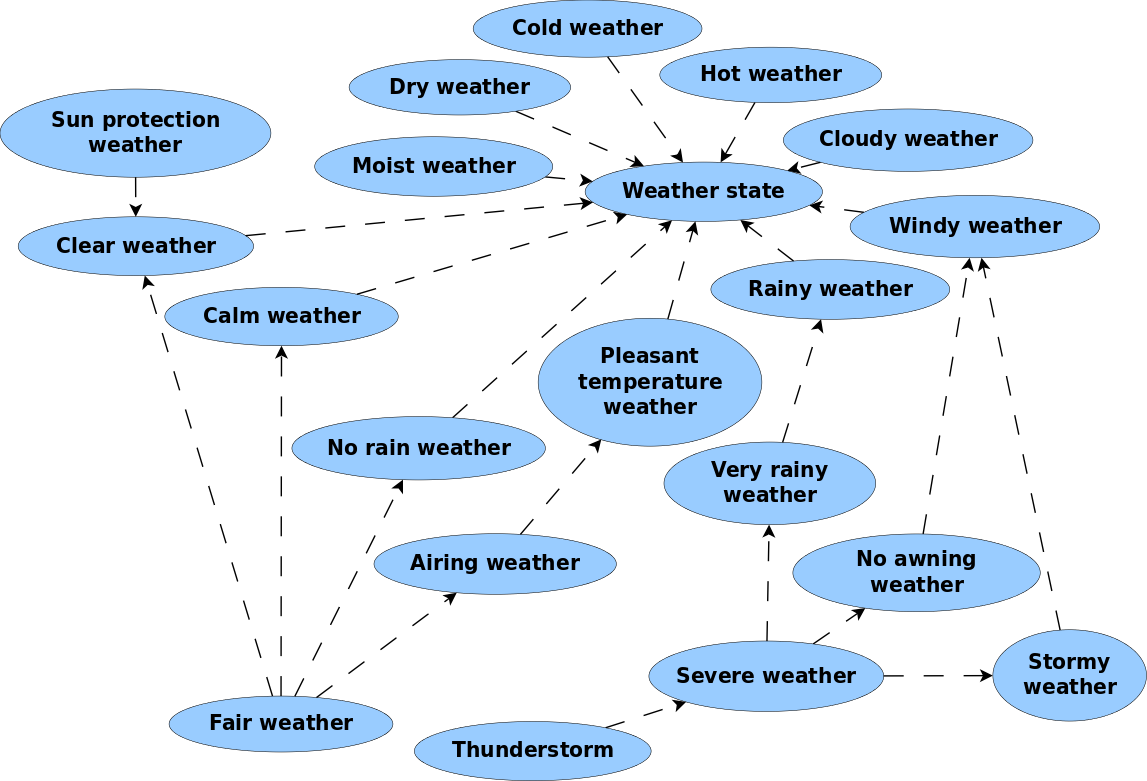
\includegraphics[width=.3\textwidth]{figures/diagrams/weather-state.png}
  \caption{Concept-classification tree for \Egls{weather state}}
  \label{fig:tree_weather_state}
\end{figure}

\subsection{Binary relations diagram}
\label{subsec:binary_relations_diagram}

The purpose of a \emph{Binary relations diagram} is to present all binary relations between concepts in the ontology (see figure~\ref{fig:binary_relations}).

% TODO add previous/next weather state
\begin{figure}
  \centering
  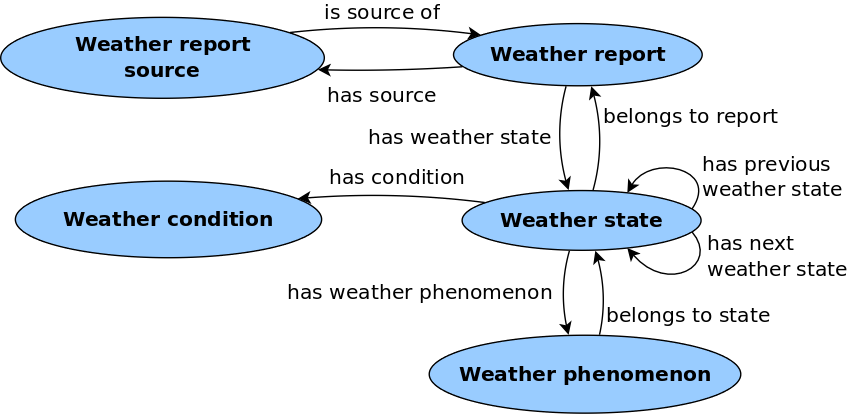
\includegraphics[width=.8\textwidth]{figures/diagrams/binary-relations.png}
  \caption{Binary relations diagram of \thinkhomeweather}
  \label{fig:binary_relations}
\end{figure}

\subsection{Concept dictionaries}
\label{subsec:concept_dictionaries}

A \emph{Concept dictionary} lists all concepts together with their names, instances, class attributes, instance attributes and relations. For the sake of clarity, this table is split up into several tables, one for each of the concept-classification trees in section~\ref{sec:concept_classification_trees}.

In the tables which can be found in the appendix in section~\ref{subsec:appendix_concept_dictionaries}, sub-concepts having the same instances, class attributes, instance attributes and relations as their super-concepts are omitted. Furthermore, any columns that are not filled with any content in any row are omitted.

\subsection{Binary relations table}
\label{subsec:binary_relations_table}

The \emph{Binary relation table} specifies all relations from section~\ref{sec:binary_relations_diagram} in detail. This includes the relations' names, their source and target concepts, their maximum source cardinalities and their inverse relations, if any. The table can be found in the appendix section~\ref{subsec:appendix_binary_relations_table}.

\subsection{Instance attributes table}
\label{subsec:instance_attributes_table}

An \emph{Instance attributes table} lists all instance attributes in \thinkhomeweather together with the concept where they belong to, their value type and value range, the unit of measurement and their cardinality. The \emph{Instance attributes table} can be found in the appendix in section~\ref{subsec:appendix_instance_attributes_table}.

\subsection{Class attributes table}
\label{subsec:class_attributes_table}

Many concepts within the \thinkhomeweather ontology define themselves to be specializations of other concepts. E.g. the concepts \Egls{very low pressure}, \Egls{low pressure}, \Egls{normal pressure}, \Egls{high pressure} and \Egls{very high pressure} are all sub-concepts of \Egls{atmospheric pressure}. They all differ by the value of the instance attribute \egls{has pressure value} that every instance of \Egls{atmospheric pressure} has.

These concepts are summarized in the \emph{Class attributes table} in the appendix in section~\ref{subsec:appendix_class_attributes}.

\subsection{Instances table}
\label{subsec:instances_table}

The only pre-defined instances in \thinkhomeweather are the instances of the concept \Egls{weather condition}. Their details can be found in the \emph{Instance table} in the appendix in section~\ref{subsec:appendix_instances_table}.

\section{Integration}
\label{sec:integration}

One of the goals when designing an ontology is to reuse existing ontologies where possible\cite{reuse1}\cite{reuse2}. It the domain of \thinkhomeweather, four areas have been identified where existing ontologies can be reused: These are location data, measurement units, weather concepts and specifications of date and time. Chapter \ref{ch:existing_work} sheds some light on existing ontologies around the domain of weather data. In this section, the ontologies that have found to be eligible for reuse within \thinkhomeweather are presented.

\paragraph{Location data:}

Each \Egls{weather report} is valid for a certain location on Earth, given by \emph{latitude}, \emph{longitude} and \emph{altitude}. To handle such location data, the \emph{W3C Semantic Web Interest Group}\footnote{\href{http://www.w3.org/2001/sw/interest/}{http://www.w3.org/2001/sw/interest/}} developed the \emph{Basic Geo (WGS84 lat/long) Vocabulary}\cite{wgs84_vocabulary}. It introduces a concept called \emph{Spatial thing} and its attributes \egls{lat}, \egls{long} and \egls{alt} according to the \emph{WGS-84 geodetic reference system}\cite{WGS84}.

However, the vocabulary contains some data properties that are incorrectly defined to be annotation properties. Thus, they must be redefined to be data properties whenever used in an ontology.

\paragraph{Weather concepts:}

The \emph{SWEET} ontology\cite{SWEET}\footnote{\href{http://sweet.jpl.nasa.gov/ontology/}{http://sweet.jpl.nasa.gov/ontology/}} developed by the \emph{Jet Propulsion Laboratory} at the \emph{California Institute of Technology}\footnote{\href{http://www.jpl.nasa.gov/}{http://www.jpl.nasa.gov/}} offers a wide range of concepts, attributes and individuals for environmental and atmospherical phenomena, including all units that may be used in weather data ontologies. \emph{SWEET} is designed in a highly modular manner; there is a single \emph{OWL} file that provides definitions of measurement units. However, any file that is part of \emph{SWEET} depends on a number of other files belonging to that ontology and these in turn have dependencies. Thus, importing one of \emph{SWEET}'s \emph{OWL} files entails the import of a large number of other files; a simple ontology like \thinkhomeweather becomes hard to handle. Hence, reusing \emph{SWEET} is not an option.

Besides \emph{SWEET}, there is no ontology providing weather concepts that has been determined to be appropriate for use in the \thinkhomeweather ontology. Hence, \thinkhomeweather defines its own weather concepts.

\paragraph{Units of measurement:}

\newcommand{\muo}{\emph{MUO}\xspace}

All instances of \egls{Weather phenomenon} have one or more attributes specifying details about the weather element that is being represented (refer to appendix~\ref{subsec:appendix_instance_attribute_tables} for details about these attributes). Each of these attributes assigns a numerical value to the \egls{Weather phenomenon}. To avoid confusion by the use of different units for one attribute (e.g. \si{\degree F} and \si{\celsius} for the \emph{Temperature value}) the unit being used shall be added to the attribute value.

As the use of units of measurement is a topic that occurs in many ontologies, there are several different approaches to cope with it.

The \emph{Measurement Units Ontology}\footnote{\href{http://idi.fundacionctic.org/muo/muo-vocab.html}{http://idi.fundacionctic.org/muo/muo-vocab.html}}\cite{MUO} is a simple and light-weight approach to enrich measurement values in an ontology with appropriate units. Some of the most important units are pre-defined, others can easily be added when needed. The \emph{Measurement Units Ontology} (\muo) is still work in progress, however it is not expected that it might change heavily in the future. Everything that will be reused by other ontologies will remain unchanged. Hence, \muo can be imported into any ontology without problems.

Besides the \emph{Measurement Units Ontology}, several other ontologies have been examined, but all of them have shortcomings that render their use in the \thinkhomeweather ontology impossible. These ontologies are:
\begin{itemize}
  \item \textbf{\emph{SWEET}}: Besides concepts, attributes and individuals for atmospherical phenomena, \emph{SWEET} also comes with support for literals more precisely specified by units. However, as mentioned above, \emph{SWEET} is an ontology that is inappropriate for use in \thinkhomeweather.
  
  \item \textbf{\emph{QUDT}}: \emph{QUDT}\footnote{\href{http://www.qudt.org/}{http://www.qudt.org/}}, a set of ontologies for \emph{Quantities, Units, Dimensions and Data Types in OWL and XML}, is a promising approach for adding support for units to an \emph{OWL} ontology. However, \emph{QUDT} does not work in \protege together with the \emph{Pellet} reasoner. Using \emph{QUDT} would require several changes to its \emph{OWL} files. Hence, it cannot be used in the \thinkhomeweather ontology.
  
  \item \textbf{\emph{QUOMOS}}: The \emph{OASIS Quantities and Units of Measure Ontology Standard} (\emph{QUOMOS})\footnote{\href{https://www.oasis-open.org/committees/tc\_home.php?wg\_abbrev=quomos}{https://www.oasis-open.org/committees/tc\_home.php?wg\_abbrev=quomos}} is a project that aims at developing ``an ontology for quantities, systems of measurement units, and base dimensions for use across multiple industries''. However, as no deliverables have been released at the time of writing, it cannot be used in \thinkhomeweather.
  
  \item \textbf{OBO Foundry Initiative}: The \emph{OBO Foundry Initiative}\footnote{\href{http://obofoundry.org/}{http://obofoundry.org/}} is an initiative that aims at collecting ontologies for use in the biomedical domain. The list of \emph{The Open Biological and Biomedical Ontologies} (abbreviated by \emph{OBO}) includes an ontology for units of measurements\footnote{\href{http://obofoundry.org/cgi-bin/detail.cgi?id=unit}{http://obofoundry.org/cgi-bin/detail.cgi?id=unit}}\footnote{\href{http://code.google.com/p/unit-ontology/}{http://code.google.com/p/unit-ontology/}}. This ontology apparently covers most of the units that are used in the \thinkhomeweather ontology. However, it lacks any documentation and hence cannot be used in \thinkhomeweather.
  
  \item \textbf{OM}: The \emph{Ontology of Units of Measure and Related Concepts} (\emph{OM})\footnote{\href{http://www.wurvoc.org/vocabularies/om-1.6/}{http://www.wurvoc.org/vocabularies/om-1.6/}}\cite{OM} is another promising approach for adding measurement units to \emph{OWL} that even provides features like the conversion between different units for the same quantities and representation and checking of formulas. It is a rather large ontology (nearly \SI{2.4}{\mebi\byte} in \emph{RDF/XML syntax}) compared to the \thinkhomeweather ontology and related to the purpose it would fulfill in \thinkhomeweather; furthermore, at the time when \cite{OM} was published, development of \thinkhomeweather had already completed. Hence, \emph{OM} was not taken into account for being used in the \thinkhomeweather ontology.
\end{itemize}

Although the \emph{Measurement Units Ontology} does come with a few shortcomings (see section~\ref{sec:implementation}), it is the ontology that has been identified to be the the one that fits \thinkhomeweather requirements best.

\paragraph{Date and time:}

The attributes \egls{has start time}, \egls{has end time} and \egls{has observation time} of the concept \Egls{weather state} need to encode date and time information in an appropriate way.

For specifying temporal properties, the \emph{World Wide Web consortium} (\emph{W3C})\footnote{\href{http://www.w3.org/}{http://www.w3.org/}} offers a \emph{working draft}\cite{w3c-process} of \emph{OWL-Time}\cite{owl-time}, a \emph{Time Ontology in OWL}. It defines the concept called \emph{TemporalEntity} that can either be an \emph{instant} or an \emph{interval}. Using appropriate attributes, the properties of a \emph{TemporalEntity} are specified. Although \emph{OWL-Time} is in the state of a \emph{working draft} since September 2006, the main concepts and attributes that will be reused by other ontologies are likely to remain unchanged in future releases of that ontology.

\vspace{1em}

Section \ref{sec:implementation} describes the reuse of the aforementioned ontologies within the \thinkhomeweather ontology in detail.

\section{Implementation}
\label{sec:implementation}

After exhaustive analysis and structuring in the previous sections, the step of implementing the ontology has become a straight-forward task.

The \thinkhomeweather ontology is implemented in OWL using \protege 4.1 together with the \emph{Pellet} \emph{OWL} 2 Reasoner. \emph{Pellet} includes \emph{Pellint}\footnote{\href{http://weblog.clarkparsia.com/2008/07/02/pellint-an-ontology-repair-tool/}{http://weblog.clarkparsia.com/2008/07/02/pellint-an-ontology-repair-tool/}}, an ontology performance tool that uses a set of patterns to find possible performance problems in an \emph{OWL} ontology. \emph{Pellint} has been used intensively to ensure it does not report any problems that could affect reasoning performance.

To ensure that the reasoning of all sub-concepts of \egls{weather phenomenon}, \egls{weather state} and \egls{weather report} works correctly, \emph{JUnit}\footnote{\href{http://junit.org/}{http://junit.org/}} is used (see section~\ref{sec:importer_tests}). Every test case loads the \thinkhomeweather ontology using the \emph{Jena framework}, adds appropriate individuals and checks using the \emph{Pellet reasoner} if reasoning is performed in the desired manner.

During implementation of \thinkhomeweather in \emph{OWL}, the identifiers of concepts, properties and instances in this document are modified by removing all space characters and concatenating all parts of the identifier using \emph{camel case}\cite{CamelCase}, e.g. \Egls{Weather state} becomes \emph{WeatherState} and \egls{has start time} becomes \emph{hasStartTime}. Hence, in the \emph{OWL} implementation, all identifiers match the regular expression \texttt{\textasciicircum[A-za-z0-9]+\$}.


\subsection{Imported ontologies}

During the implementation step, the ontologies listed in section \ref{sec:integration} need to be imported and integrated. Their use necessitates the application of certain patterns required by these ontologies.

\vspace{1em}

\emph{OWL-Time}\cite{owl-time} defines the concept \egls{temporal entity} and its sub-concepts \egls{instant} and \egls{interval}, both having a self-explanatory name. The properties \egls{has start time}, \egls{has end time} and \egls{has observation time} of \egls{weather report} represent instants; however, only \egls{has observation time} is implemented to link an instance of \egls{instant} to a \Egls{weather report}. For \egls{start time} and \egls{end time}, instances of \egls{interval} are used. Such an instance represents the interval between the \egls{observation time} and the time the \Egls{weather report} is valid from/until (in hours). This simplifies reasoning of the sub-concepts of \Egls{weather report} which depend on the report's \egls{start time}; e.g. an instance of \emph{Forecast 1 hour weather report} can be defined as an instance of \Egls{weather report} having a \egls{start time} of \num{1} (hours).

Figure~\ref{fig:owl_time1} shows a \Egls{weather report} together with its with \egls{start time} and \egls{end time}; figure~\ref{fig:owl_time2} displays a \Egls{weather report} together with its \egls{observation time}. The \emph{Time Zone Ontology} that comes with \emph{OWL-Time} is not used by \thinkhomeweather. All times are given in \emph{UTC}.

\begin{figure}
  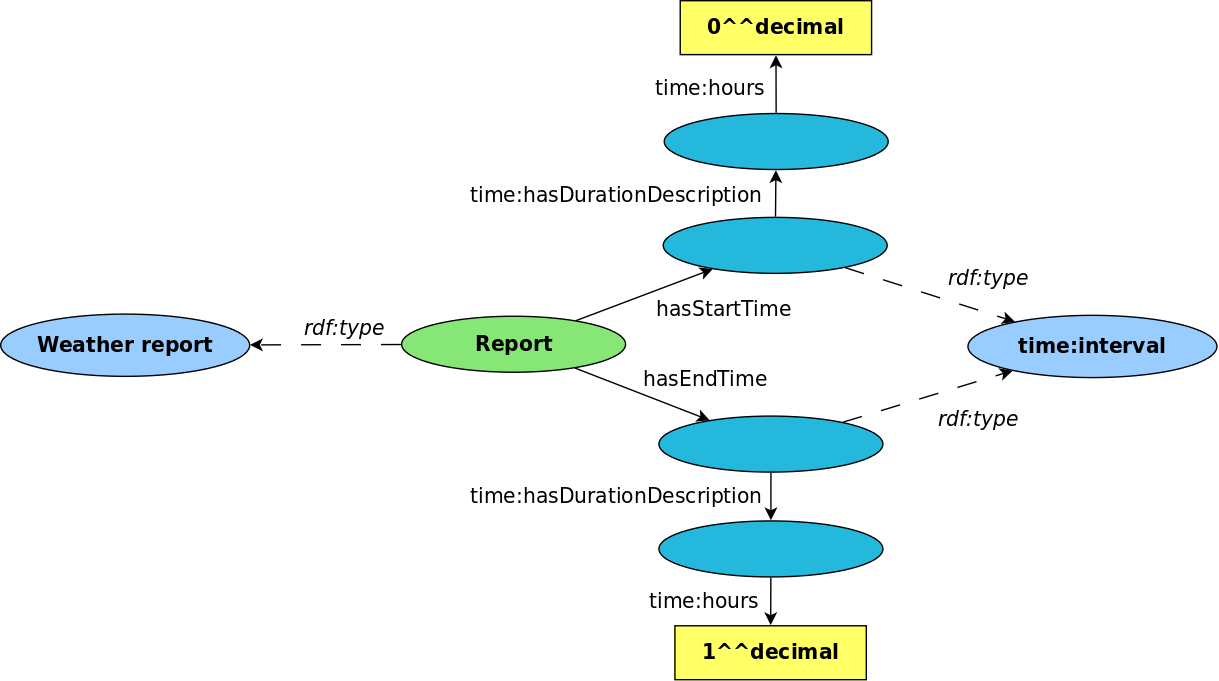
\includegraphics[width=\textwidth]{figures/diagrams/owl-time1.png}
  \caption{An instance of \Egls{current weather report} together with \egls{start time} and \egls{end time}.}
  \label{fig:owl_time1}
\end{figure}

\begin{figure}
  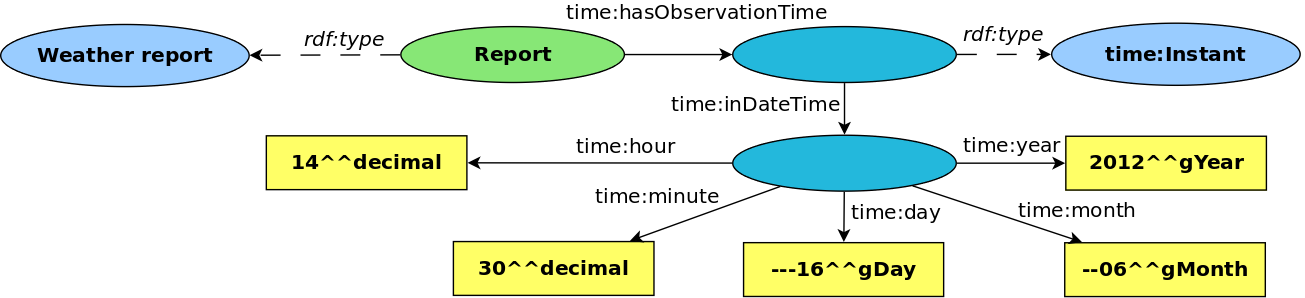
\includegraphics[width=\textwidth]{figures/diagrams/owl-time2.png}
  \caption{An instance of \Egls{weather report} together with its \egls{observation time} (\texttt{2012-06-16~14:30}).}
  \label{fig:owl_time2}
\end{figure}

\vspace{1em}

Figure~? shows how an instance of \Egls{temperature} would be implemented if no ontology for units of measurements would be used. With the introduction of the \emph{Measurement Units Ontology} (\muo), the data property and the literal are removed; an object property that is a sub-property of \emph{Quality value} (which is defined by \muo) takes the place of the data property. It links to a blank node which in turn has two properties: \emph{Measured in} and \emph{numericalValue}. The property \emph{Measured in} is an object property that refers to the unit being used which is represented by an instance of \muo's concept \emph{Unit of measurement}. Using the data property \emph{numericalValue}, the literal is connected to the blank node. The resulting pattern is seen in figure~?. % TODO reference figures

\muo is an ontology that is easy to implement in an already-existing ontology. Its major drawback in the case of \thinkhomeweather is that it affects reasoning time negatively. Repeated tests showed that reasoning time increased by about $30 \%$ when introducing \muo. However, the slowdown caused by \muo is accepted in favour of the usage of units of measurement.

\vspace{1em}

Figure~\ref{fig:owl_wgs84} shows how the \egls{location} of a \Egls{weather report} is encoded.

\begin{figure}
  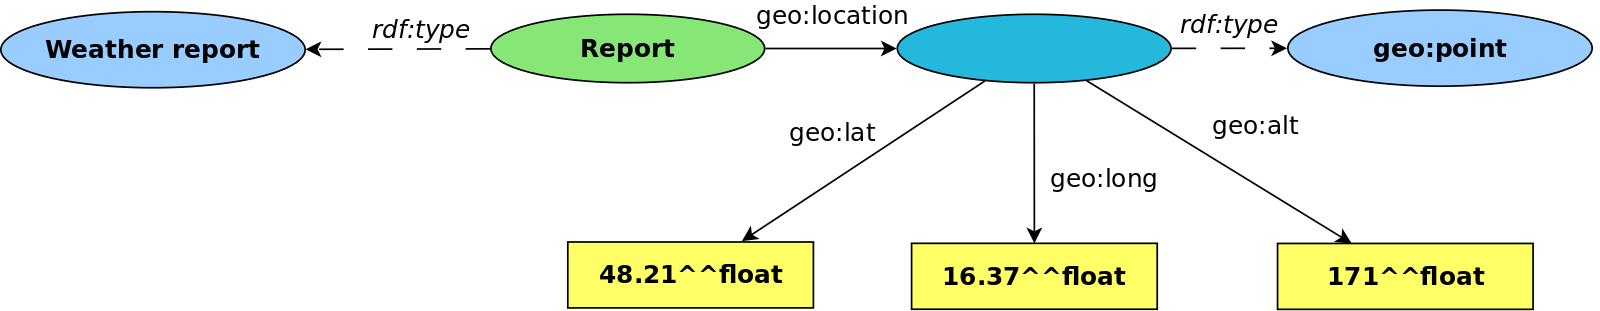
\includegraphics[width=\textwidth]{figures/diagrams/wgs84.png}
  \caption{An instance of \Egls{weather report} together with its \egls{location} (Vienna, Austria: N~\SI{48.21}{\degree}, E~\SI{16.37}{\degree}, \SI{171}{\metre} above \emph{MSL}).}
  \label{fig:owl_wgs84}
\end{figure}

\section{Evaluation}
\label{sec:ontology_evaluation}

After completing the implementation step, this section evaluates \thinkhomeweather regarding all non-functional requirements (section~\ref{sec:evaluation_non_functional}) and functional requirements (section~\ref{sec:evaluation_functional}) from section~\ref{sec:weather_information} and the \emph{Ontology Requirements Specification Document} in section~\ref{sec:ontology_specification}.

\subsection{Non-functional requirements}
\label{sec:evaluation_non_functional}

There are three non-functional requirements:

\begin{itemize}
  \item \textbf{Naming conventions}: All identifiers in \thinkhomeweather follow the naming conventions stated in section~\ref{sec:ontology_conventions}.
  \item \textbf{Documentation}: Due to following the \methontology approach, the ontology is well documented at every stage of development.
  \item \textbf{Usage of other ontologies}: \thinkhomeweather uses the \emph{Basic Geo (WGS84 lat/long) Vocabulary}, \muo and \emph{OWL-Time}; no ontology has been found that satisfies the requirements of \thinkhomeweather regarding concepts for weather data.
\end{itemize}

Thus, all non-functional requirements are met by \thinkhomeweather.

\subsection{Functional requirements}
\label{sec:evaluation_functional}

\thinkhomeweather meets its functional requirements if it provides answers to all competency questions. This section evaluates if answers are provided and how answers can be drawn from the ontology.

For the following questions, \thinkhomeweather can give straight answers:
\begin{itemize}
  \item What is the current weather situation?
  \item What will the weather situation be in one hour, in two hours, …, in 24 hours?
  \item What is the current temperature, humidity, wind speed, …?
  \item What will be the temperature, humidity, wind speed, … in one hour, in two hours, …, in 24 hours?
  \item Does it rain?
\end{itemize}
To answer any of these questions, the relevant instance of \Egls{weather report} must be identified. Via the property \egls{has weather state}, an instance of \Egls{weather state} is connected to it; this instance has in turn an arbitrary number of \egls{has weather phenomenon} properties each linking to an instance of \Egls{weather phenomenon}. The information from these instances of \Egls{weather phenomenon} provide the desired answer.

However, there are questions that cannot be answered by \thinkhomeweather as writing rules to infer answers would be too complicated in \emph{OWL}:
\begin{itemize}
  \item Will the weather change? Will the temperature, humidity, … rise or fall?
  \item Do we need to irrigate the garden?
\end{itemize}

Furthermore, there are questions that cannot be answered using an \emph{OWL} ontology due to the \emph{Open World Assumption} (\emph{OWA})\cite{open-world-assumption}. For instance, an \emph{OWL} reasoner cannot determine that some attribute value is the lowest one as it does not know whether there may be lower value it does not know anything about; the reasoner only knows about the presence of individuals and attribute values, but nothing about their absence.

\begin{itemize}
  \item What will be the minimum temperature, humidity, … over the next 24 hours? What about maximum values?
  \item Will it rain in the next hours? Will it rain today?
  \item Will there be sunshine today?
  \item Will there be severe weather?
  \item Will temperature drop/stay below \SI{0}{\celsius}?
  \item When can we open windows and when do we have to keep them shut?
  \item When do we need sun protection?
  \item When will it outside be colder than inside the house? When will it be warmer?
\end{itemize}

However, for each of the above competency questions, whether a direct answer can be given or not, \thinkhomeweather can provide all available data; an external program that does not rely on the \emph{Open World Assumption} can access this data and generate an answer.

Hence, the ontology constructed in this chapter complies with its specification in section \ref{sec:ontology_specification}.
